%\documentclass[12pt]{article}

%\usepackage[pdftex]{graphicx}

%\begin{document}



\chapter{NuSIM Coordinate Systems Database}
%\author{Isaac Sheff}
%\maketitle
%\newpage
%\tableofcontents
%\newpage
\section{Purpose}
The various components of NuSIM each operate in their own coordinate systems, and so in order to simulate the entirety of the spacecraft, it is necessary to keep track of the transformations between these systems. Furthermore, for many tests it is necessary to simulate NuSIM under changing conditions, and so for each timestep a set of coordinate system transformations must be provided. 

\subsection{List of Coordinate System Transformations}


\begin{tabular}{| r | l |}
\hline
{\bf Name}	&	{\bf Transformation}						\\
\hline
Inertial-SC	&	Inertial Frame to Spacecraft				\\
SC-FB		&	Spacecraft to Focal Bench				\\
FB-FP0		&	Focal Bench to First Focal Plane Module		\\
FB-FP1		&	Focal Bench to Second Focal Plane Module	\\
FB-MD0		&	Focal Bench to First Metrology Detector		\\
FB-MD1		&	Focal Bench to Second Metrology Detector	\\
FB-AS0		&	Focal Bench to First Aperture Stop			\\
FB-AS1		&	Focal Bench to Second Aperture Stop		\\
FB-OB		&	Focal Bench to Optics Bench (the mast)		\\
OB-OM0		&	Optics Bench to First Optics Module			\\
OB-OM1		&	Optics Bench to Second Optics Module		\\
OB-ML0		&	Optics Bench to First Metrology Laser		\\
OB-ML1		&	Optics Bench to Second Metrology Laser		\\
OB-ST		&	Optics Bench to Star Tracker				\\
\hline
\end{tabular}


\section{Format}
In order to provide NuSIM with a set of coordinate system transformations for each time step, a comma separated values (.csv) spreadsheet is used.
\subsection{Layout}
Each time-step is a pair of sequential rows: one for the translation between the coordinate systems, presented in (x, y, z), and the other for the rotation, presented as a quaternion, with the real component last: (q1, q2, q3, q4). Thus each coordinate system transformation is a set of four adjacent columns, and on the first row of each time-step the fourth column of each coordinate system transformation is empty. 

There are several rows before the time-steps begin, representing header data at the top of the database file. These will include a row in which the name of each coordinate system transformation is in the first of the four columns its values occupy. 

There are no rows between the time-steps, and no rows of interest after the time-steps. 

\subsection{Template}
With each database format revision, a template file is produced, often in microsoft excel format. This file is simply a database with a single time-step: all the components in their ideal configuration. Historically, these file have been named along the lines of ``NuSIM\_OrientationsIDEAL\_005.xls." Note that while Microsoft Excel's exported CSV files use carriage return (``\textbackslash r") line-breaks, NuSIM requires its input databases to use newline (``\textbackslash n") line-breaks. 

\subsection{Diagrams}
\subsubsection{File Layout}
\begin{tabular}{| c | c | c | c | c |}
\hline
\multicolumn{5}{| c |}{ }\\
\multicolumn{5}{| c |}{\Large Header}\\
\multicolumn{5}{| c |}{ }\\
\hline
 & & & & \\
{extra header info} & Inertial-SC & SC-FB & {\Huge \ldots} & OB-ST\\
 & & & & \\
{\Huge $\Downarrow$} & {\Huge $\Downarrow$} & {\Huge $\Downarrow$} & {\Huge $\Downarrow$} & {\Huge $\Downarrow$}\\
  & & & & \\
\hline
\end{tabular}

\subsubsection{column layout}
\begin{tabular}{| c || l | l | l | l |}
\hline
{\bf Section} & \multicolumn{4}{ c |}{\bf Content}\\
\hline
 & \multicolumn{4}{ c |}{ }\\
 & \multicolumn{4}{ c |}{ header info}\\
 & \multicolumn{4}{ c |}{ }\\
\cline{2-5}
Header & Name & & & \\
\cline{2-5} 
 & \multicolumn{4}{ c |}{ }\\
 & \multicolumn{4}{ c |}{ more header info}\\
 & \multicolumn{4}{ c |}{ }\\
\hline
Time- & $x$  translation & $y$ translation & $z$ translation & \\
\cline{2-5}
Step 0 & $q_1$ ($i$ coefficient) & $q_2$ ($j$ coefficient) & $q_3$ ($k$ coefficient) & $q_4$ (real)\\
\hline
Time- & $x$  translation & $y$ translation & $z$ translation & \\
\cline{2-5}
Step 1 & $q_1$ ($i$ coefficient) & $q_2$ ($j$ coefficient) & $q_3$ ($k$ coefficient) & $q_4$ (real)\\
\hline
Time- & $x$  translation & $y$ translation & $z$ translation & \\
\cline{2-5}
Step 2 & $q_1$ ($i$ coefficient) & $q_2$ ($j$ coefficient) & $q_3$ ($k$ coefficient) & $q_4$ (real)\\
\hline
 & & & & \\
 \multicolumn{1}{| c ||}{\Huge $\Downarrow$} & \multicolumn{1}{ c |}{\Huge $\Downarrow$} &  \multicolumn{1}{ c |}{\Huge $\Downarrow$} &  \multicolumn{1}{ c |}{\Huge $\Downarrow$} &  \multicolumn{1}{ c |}{\Huge $\Downarrow$}\\
  & & & & \\
  \hline
\end{tabular}

\section{NuSIM Database Transformer}
NuSIM Database Transformer is a python library meant to simplify the process of generating multiple time-step databases with algorithmically generated coordinate system transformations. It takes as input the ideal template database (in csv format), and outputs sequential steps in accordance with an input function. 

\subsection{Requirements}
	NuSIM Database transformer is a Python script. That means it 
requires an installation of Python to run. Python comes standard on most 
modern Linux installations as well as OSX (although it may be in the 
developer tools, I don't recall), and is available free for most any 
operating system (even Windows) from python.org. To check to see if you 
have python, enter into a terminal:
\begin{verbatim}
	python
\end{verbatim}
If you find yourself in a python shell, you've got python. Exit with:
\begin{verbatim}
	exit()
\end{verbatim}
	You do need to be able to program in Python to use NuSIM Database 
Transformer. Python is an interpreted language conforming to a number of 
common standards, which allows for mostly iterative programming with the 
ability to create functional (using functions themselves as variables) and 
object oriented programming. This readme talks about python objects,
functions, lambdas, tuples, lists, and dictionaries. Tutorials and 
explanations are available at python.org

	NuSIM Database transformer requires an ideal database in CSV 
format. It assumes that this database contains the entries:
\begin{verbatim}
	'Inertial-SC','SC-FB','FB-FPM0','FB-FPM1','FB-MD0','FB-MD1',
	'FB-AS0','FB-AS1','FB-OB','OB-OM0','OB-OM1','OB-ML0','OB-ML1',
	'OB-ST'
\end{verbatim}
All on the same row, and that the last two rows with numbers in them are 
the ideal translational coordinates and the ideal rotational quaternians, 
respectively. Furthermore, it expects each transformation name listed above 
to share a column with the first of the three adjacent translational 
coordinates and the first of the four adjacent quaternion components (which 
are stored constant last, by the way). This is the standard format as found 
in ideal databases 005 and 006, and the database can handle any other extra 
columns, rows, or comments inserted into the ideal database as long as 
these rules are adhered to. 

\subsection{Description}
	NuSIM Databse Transformer is simply a python library containing 
useful tools for the generation of parametrically-changing databases for 
NuSIM. These are:

\subsubsection{arcsecondsToRadians(asec)}
returns asec, but in radians.

\subsubsection{eulerAnglesToQuaternion(xrot, yrot, zrot)}
	Converts euler angles to quaternions via the formula from \newline
http://en.wikipedia.org/wiki/Conversion\_between\_quaternions\_and\_Euler\_angles 
according to the x-y-z convention, which is the same as the formula from 
"Quaternions and Rotation Sequences" by Jack B. Kuipers, page 207, for 
converting Aerospace angle sequences to Quaternions. This means that  what 
we are doing here is technically rotating about Z, then Y, then X. There is 
a small change in convention here; because we are doing a  frame rotation, 
and not a point rotation, we are reversing the coefficient terms (hence the 
(-1.0)*), and we are putting the constant term last instead of first. It 
returns these as a tuple with four entries. 

\subsubsection{Class Output\_Writer}
	A simple class which will either print or write to a file depending 
on what you want to do.  If no filename, or a filename of None is 
input, .write() prints out (sans newlines or space each time), but if a 
filename is input, then .write() writes to that filename. close does 
nothing if you are printing out, but it closes the file if you're writing a 
file.

	Database (described below) writes with one of these so it is 
possible to run a script that writes a database and pipe it somewhere 
instead of writing immediately to a file.

\subsubsection{Class Entry}
	Each entry in the database needs a quaternion (.quater) with 4 
entries and a set of coordinates (.coords) with three entries. These can be 
set directly be inputting a tuple into setCoords or  setQuatr, or by 
inputing 3 numbers into setCoords and 4 into setQuatr. The inputs to the 
Constructor are the same as the inputs to setCoordsAndQuatr, which is to 
say either all three coords followed  by all four entries of the quatr, or 
two tupples in a row.  getX, getY, getZ, and getQ1, getQ2, getQ3, getQ4 are 
self explanatory keep in mind that the last entry of our quaternions is the 
constant term, (getQ4)


\subsubsection{Class Database}
	This is the REALLY USEFUL ONE. This is a class designed to facilitate the creation of 
	database files as input for NuSIM. This class takes as 
	constructor input a filename of an ideal file.

	After construction, a Database object has the following fields:
	
\begin{itemize}
\item 	newline:	 the newline character (either \textbackslash n or \textbackslash  r
				which this should use when writing a .csv
\item		desiredColumns:	the list of all the column names to use in
				this database
\item		header:		the text part of the database above the 
				timesteps
\item		columns:	the dictionary of all the column names as 
				keys for their x coordinate in the .csv
\item		ideal:		the ideal Entry objects read form the ideal 
				database (with column names as keys)
\item		current:	the current Entry objects read form the 
				ideal database (with column names as keys)
\item		previous:	the previous Entry objects read form the 
				ideal database (with column names as keys)
\item		idealCoordsLine:	the coordinates line (split by ",") 
					which was read from the ideal 
					database
\item		idealQuaterLine:	the quaternions line (split by ",") 
					which was read from the ideal 	
					database
\item		step:		the current timestep (starts at 0)
\item		out:		the Output\_Writer object with which to 
				write out the .csv
\end{itemize}

	This means that you can get, for example, the current X coord of 
	FB-OB with:
	\begin{verbatim}
		database.current['FB-OB'].getX()
	\end{verbatim}
	Writing functions:
\begin{itemize}
\item		open(filename):
			this function sets this object to write at the
			given filename. It does this by setting 
			self.out to be an Output\_Writer(filename), so you 
			can fail to put in a filename and write to 
			standard out.

\item		close():
			call this when this Database is done writing.

\item		writeHeader():
			writes the self.header to out. Do this first when 
			writing a database,

\item		writeStep()
			writes the current Step, exactly as formatted in 
			idealCoordsLine and idealQuaterLine, but with the 
			information from current, to out.


\item		newStep(stepFunc):
			This is the really important one. 
			This function creates a new step, sets previous 
			step to current step, and current to new step.
			There are two things you can enter into newStep:
		\begin{itemize}
			\item	 any function with input (this database
				   object) that outputs the next step
				   If you input to newStep any function 
				   that returns a dictionary with valid
				   Entry objects keyed to every entry of 
				   desiredColumns, when given this database 
				   object as input (as in, newStep calls 
				   stepFunc(self)), newStep will happily 
				   make the new Step the one setpFunc 
				   output. 
	
			\item any dictionary of functions which output entries
			   keyed to any subset of desiredColumns
			   for example, if I only wanted to play with FB-OB
			   and SC-FB, I'd:
\begin{verbatim}
database.newStep({
	'FB-OB':function_that_given_input_database_outputs_entry_for_FB-OB,
	'SC-FB':function_that_given_input_database_outputs_entry_for_SC-FB
		})
\end{verbatim}
		\end{itemize}
	
						 
\item		writeDatabase(steps, stepFunc, output\_filename):
			simply starts a database at output\_filename, writes
			the header there, and writes steps Steps to 
			The database, iterating each time with stepFunc, 
			and then closes the database.
\end{itemize}

\subsection{Use}
	To use NuSIM Database Transformer, a python script needs to import 
it as a library. Then it can use the tools listed above, which should be 
helpful in generating varying parameter databases for NuSIM. 

	The most useful single method of the library is:
Database.writeDatabase(steps, stepFunc, output\_filename).

	To use this, create a database object (remember that the Database 
constructor takes as input the name of an ideal database CSV file), and 
then call the writeDatabase method from that object. The inputs should be:
\begin{itemize}
\item		steps:	the number of steps this database should have
\item		stepFunc:	This can be either a function, which given 
			a database object input, returns a dictionary with 
			Entry objects  keyed to each of: 'Inertial-SC','SC-
			FB','FB-FPM0','FB-FPM1','FB-MD0','FB-MD1','FB-
			AS0','FB-AS1', 'FB-OB','OB-OM0','OB-OM1','OB-
			ML0','OB-ML1', and 'OB-ST', or a dictionary 
			containing a subset of the above keys, each keying 
			to a function that takes a database object as input 
			and returns an Entry object. 
			This is the function with which the next step of 
			the database will be computed at each step. 
\item		output\_filename:	the name of the file you want to 
			write this database to. This will be a csv file in 
			the same format as the ideal file the Database 
			object was created with. This can be NULL if you 
			want to just print it. 
\end{itemize}
	Recall that python functions can be declared anonymously (inline) 
in the following format:
\begin{verbatim}
	lambda inputs: output
\end{verbatim}
Using this, it is possible to write a multi-step database in as little as 
one line of Python (although for readability this is inadvisable. 

	Remember that once a Database object has written, it increments its 
current step and resets its current and previous step entries. Therefore, 
writing multiple times from one Database object produces a continuation of 
the database, possibly with varying stepFunc entries, or multiple files. If 
you want to write multiple different databases from one ideal database, it 
is easiest to use the copy library, and after creating a database object 
from an ideal database, copy.deepcopy() it each time you want a database 
object to write with. 

	To run a python script you've written using this or any other library,
call from a terminal:
\begin{verbatim}
	python script.py
\end{verbatim}

\subsection{Examples}
	Note that readme\_nusim\_database\_transformer.py is a text-only copy of this section of this document written as executable python. Running it will run all these examples. 



\subsubsection{Importing}
	The first step to using the NuSIM Database Transformer library is 
to import it. Python allows for 
\begin{verbatim}
	import nusim_database_transformer
\end{verbatim}
but this would mean we'd have to type
\begin{verbatim}
	nusim_database_transformer.
\end{verbatim}
before everything we used that was defined in the library. For example, 
we'd have:
\begin{verbatim}
	db = nusim_database_transformer.Database("ideal_file.csv")
\end{verbatim}
This is a pain. Therefore we will simply import everything in the library 
into the script:
\begin{verbatim}
from nusim_database_transformer import *
\end{verbatim}

\subsubsection{Create a Database Object}
Next we have to make a database object. Here it is important to choose the 
input file which is of the correct format. The one we've been using 
recently as of the time of this writing is called ``NuSIM\_OrientationsIDEAL\_005.csv"
And so we create a database object from that ideal file:
\begin{verbatim}
db = Database("NuSIM_OrientationsIDEAL_005.csv")
\end{verbatim}
If at some future date, we wanted database files computed from the ideal 
database ``NuSIM\_OrientationsIDEAL\_006.csv", we would simply have written:
\begin{verbatim}
db = Database("NuSIM_OrientationsIDEAL_006.csv")
\end{verbatim}
instead, and that would have been the only difference in the script. 


\subsubsection{Simple Database}
Now it is time to think about what we'd like to write to our output 
databases. 

Consider the simplest case: a database consisting of all ideal entries. 
This allows for a simple illustration of the writeDatabase method.

The most powerful input for newStep or writeDatabase is stepFunc: any
function, which given the entire database object, can manipulate that
object and return a dictionary representing the next step, computed
in any possible fashion.

The simplest possible value for stepFunc here would be a function that 
given an input database returned exactly the ideal step every time:
\begin{verbatim}
def simpleStepFunc(database):
      return database.ideal
\end{verbatim}
Now, remember that a single database object should not be used to write 
more than one database file, as it will always write a continuation of the 
steps it has hitherto been writing (the step number always increments), so 
it is convenient, rather than generating a new database object each time we 
want to write a database, to copy the one we have, and write from the copy.
\begin{verbatim}
import copy
db2 = copy.deepcopy(db)
\end{verbatim}
To write a database of 100 steps to the file ``100\_ideal\_steps\_A\_005.csv", 
we'd call:
\begin{verbatim}
db2.writeDatabase(100, simpleStepFunc, "100_ideal_steps_A_005.csv")
\end{verbatim}
Furthermore, recall that using inline functions, this can be done in 
fewer lines:
\begin{verbatim}
db3 = copy.deepcopy(db)
db3.writeDatabase(
            100, lambda database: database.ideal, 
            "100_ideal_steps_B_005.csv"
            )
\end{verbatim}

In addition, remember that it is also possible to substitute for stepFunc a 
dictionary of Entry - returning functions for each entry you want to vary 
with each step. The current step is initialized to be the ideal step, and 
so we, in effect, simply do not wish to vary any entries. We can therefore 
input for stepFunc an empty dictionary:
\begin{verbatim}
db4 = copy.deepcopy(db)
db4.writeDatabase(100, {}, "100_ideal_steps_C_005.csv")
\end{verbatim}


\subsubsection{Constant Offset}
Now consider a slightly more complicated case: 
We want a database of 100 entries which are all the same, but not ideal. 
For example, consider the case where FB-OB is shifted along x by 5 mm.
Here we need simply change the current step, and then print out 100 steps 
which are all unchanged from the current step.
The clearest (if not the absolute shortest, codewise) way to accomplish 
this is:
\begin{verbatim}
db5 = copy.deepcopy(db)
db5.current['FB-OB'] = Entry(
                            db5.current['FB-OB'].getX() + 5,
                            db5.current['FB-OB'].getY(),
                            db5.current['FB-OB'].getZ(),
                            db5.current['FB-OB'].getQ1(),
                            db5.current['FB-OB'].getQ2(),
                            db5.current['FB-OB'].getQ3(),
                            db5.current['FB-OB'].getQ4()
                 )
db5.writeDatabase(100, {}, "100_FB-OB_x+5_A_005.csv")
\end{verbatim}

\subsubsection{Translations}
Next, let's move on to somewhat more practical applications. 

For example, consider shifting the x translation of FB-OB by 1 mm each 
step. You could add 1 to the current step each time:
\begin{verbatim}
def add1mmToX(database):
    return Entry(
                database.current['FB-OB'].getX() + 1.0,
                database.current['FB-OB'].getY(),
                database.current['FB-OB'].getZ(),
                database.current['FB-OB'].getQ1(),
                database.current['FB-OB'].getQ2(),
                database.current['FB-OB'].getQ3(),
                database.current['FB-OB'].getQ4()
             )

db6 = copy.deepcopy(db)
db6.writeDatabase(
                    100, 
                    {
                        'FB-OB':add1mmToX
                    }, 
                    "100_FB-OB_x+n_A_005.csv"
                 )
\end{verbatim}



\subsubsection{Rotations}
Let's say you wanted to test how NuSIM reacts under various rotations about 
x, 0.1 arc seconds each step, between the optical bench and the focal 
bench, without any translation. 

Recall than an Entry constructor can accept a pair of tuples, one for 
coordinates and one for quaternions. 
\begin{verbatim}
def rotationsStepFunction(database):
    return Entry(
            database.current['FB-OB'].coords,
            eulerAnglesToQuaternion(
                                    arcsecondsToRadians(0.1*database.step),
                                    0.0,
                                    0.0
                                    )
             )

db7 = copy.deepcopy(db)
db7.writeDatabase(
                    100, 
                    {
                        'FB-OB':rotationsStepFunction
                    }, 
                    "100_FB-OB_xrot+n_A_005.csv"
                 )
\end{verbatim}

\section{Thermal Mast Bending}

The document ``Thermal\_Distortion\_2\_for\_JPL.xlsx" details the effects on the mast under the thermal effects of sunlight. In particular, it provides $x$ and $y$ offsets of the focal plane intersections with the beams from the optics, as well as $rotZ$, the twisting of the mast itself. These effects are most pronounced for a 170 degree angle of the mast toward the sun. To more fully model the effects of thermal mast bending on NuSTAR, a coordinate system transformation database had to be constructed for the mast in the configurations predicted for a full orbit. 


\subsection{Modeling the Mast as an Arc}

The data given for mast distortions due to heating is given as a set of data points for different positions relative to the sun, with each point composed of the displacement of the beams from the optics modules at the focal bench, as well as the rotation (twist) of the mast itself. 

I operated under the following assumptions:

\begin{itemize}
    \item The twist in the mast is small enough that its effect on the bend of the mast is not worth calculating, which is to say it can be interpreted as one of the benches at either end having been rotated about the mast.
    \item The mast bend in $x$ and $y$ dimensions can be interpreted as separate arcs, and the displacement from each is additive, as the mast is square and is likely to bend more or less independently in each direction along these small angles. 
    \item The beams from the optics modules are meant to move exactly parallel to the mast, centered at the center of the OM coordinate system. (supported by the coordinate systems IDEAL reference documentation).
    \item Over these small angles, second order approximations of cosine are acceptable. 
\end{itemize}

First of all, I had to translate the coordinates given for the distortion of $x$ and $y$ along the rotated (by ROTZ) focal plane into distortions of $x$ and $y$ in a plane not rotated along $z$ with respect to the optics modules. 

This is most easily done by converting to radial coordinates with the center being the mast, and subtracting $ROTZ$ from the angle.

\[
r = \sqrt{x^2+y^2}
\]
\[
\theta = \arctan \left(\frac{x}{y}\right)
\]
\[
correctedY = r \sin \left(\theta-ROTZ\right)
\]
\[
correctedX = r \cos \left(\theta-ROTZ\right)
\]

Now that those are corrected, we need to calculate the arc of the mast.

Let $m$ be the length of the mast itself, which is mostly invariant, so we shall consider this to be the arc length. The arc angle $\theta$ and the arc radius $r$ can be determined as follows:

The mast is essentially an arc (of radius $r$) with the optics module and the exact point on the focal plane meant to receive it each on what amount to beams perpendicular to the arc extending out by a distance $x$. Since the distortions in $x$ and $y$ are positive in all cases, we can assume the center of the arc is on the opposite side of NuSTAR from the $+X$ detector. Therefore the line from the center of the arc to the optics module emitting the beam (length $r+x$) is a leg of a right triangle, with the other leg being the beam itself and the hypotenuse being the line from the center of the arc to the point where the beam hits the detector (length $r+x+\Delta x$).
\subsubsection{Mast Bending Model Diagram }
\begin{center}
\leavevmode
%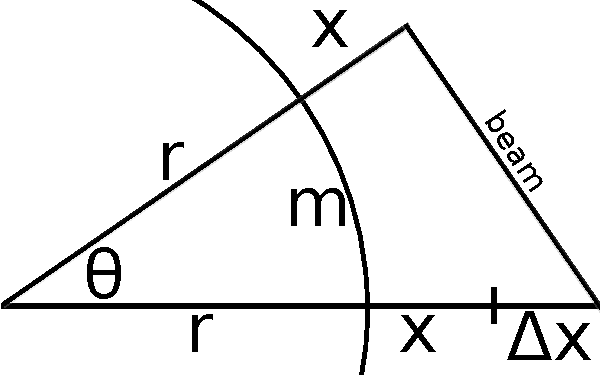
\includegraphics[width=0.8\textwidth]{mast_bending_model.pdf}
\end{center}


 Thus:
\[
\cos \left( \theta \right) = \frac{r+x}{r+x+\Delta x}
\]
A general rule of arcs is:
\[
m = \theta r
\]
So:
\[
\cos \left( \theta \right) = \frac{\frac{m}{\theta}+x}{\frac{m}{\theta}+x+\Delta x}
\]
This is not solvable analytically, (or at least Mathematica couldn't), so here we shift to a second order approximation of $\cos$, which should be accurate for these small angles:
\[
1-\frac{\theta^2}{2} \approx \frac{\frac{m}{\theta}+x}{\frac{m}{\theta}+x+\Delta x}
\]
For which the solutions for $\theta$ are:
\[
\frac{-m \pm \sqrt{m^2+8x\Delta x + 8{\Delta x}^2}}{2 \left( x + \Delta x \right)}
\]
Given that when $\Delta x = 0$, $\theta = 0$, the correct solution is:
\[
\frac{-m + \sqrt{m^2+8x\Delta x + 8{\Delta x}^2}}{2 \left( x + \Delta x \right)}
\]
Which does indeed grow as expected as $\Delta x$ grows, so it seems a reasonable solution. 


Given $\theta$, and $r = \frac{m}{\theta}$, It should be clear that the optics bench will move by $r\left(1-\cos\left(\theta\right)\right)$ along the $x$ axis and $r\sin\left(\theta\right)-m$ along the $z$ axis. 

The optics bench itself, if we are looking at the arc with $x$ translation, will rotate by $\theta$ about $y$. 

The two dimension of bend ($x$ and $y$) are essentially the same, and each is calculated as above, with their effects considered additive. 

\subsection{Implementation}
A Coordinate System Transformation database was generated for each of the bent mast positions given by the original data using the NuSIM Database Transformer Python library. The function used to compute the transformation between the focal bench and the optical bench (the mast, ``FB-OB") was as follows:

\begin{verbatim}
def compute_bent_mast_step(database):
    global thermals  # a list of (deltaX0, deltaY0, deltaX1, deltaY1,rotZ) 
    x = database.ideal["OB-OM1"].getX()+database.ideal["FB-OB"].getX()
    y = database.ideal["OB-OM1"].getY()+database.ideal["FB-OB"].getY()
    rotZ = float(thermals[database.step][4])
    m=database.ideal["FB-OB"].getZ()+database.ideal["OB-OM1"].getZ()-
        database.ideal["FB-AS1"].getZ()
    deltaX = 25.4*thermals[database.step][0]
    deltaY = 25.4*thermals[database.step][1]
    rotR = math.sqrt((x**2) + (y**2))
    rotBase = math.atan(y/x)
    x = rotR*math.cos(rotBase - rotZ)
    y = rotR*math.sin(rotBase - rotZ)
    x_mast_arcangle = ((-1.0*m)+math.sqrt((m**2.0)+(8.0*x*deltaX)+
        (8.0*(deltaX**2.0))))/(2.0*(x+deltaX))
    x_mast_arcradius = m/x_mast_arcangle
    x_translation = x_mast_arcradius*(math.cos(x_mast_arcangle)-1.0)
    x_component_z_translation = 
        (x_mast_arcradius*math.sin(x_mast_arcangle))-m
    y_mast_arcangle = ((-1.0*m)+math.sqrt((m**2.0)+(8.0*y*deltaY)+
        (8.0*(deltaY**2.0))))/(2.0*(y+deltaY))
    y_mast_arcradius = m/y_mast_arcangle
    y_translation = y_mast_arcradius*(math.cos(y_mast_arcangle)-1.0)
    y_component_z_translation = 
        (y_mast_arcradius*math.sin(y_mast_arcangle))-m
    return Entry((
                    database.ideal["FB-OB"].getX() + x_translation,
                    database.ideal["FB-OB"].getY() + y_translation,
                    database.ideal["FB-OB"].getZ() + 
                        x_component_z_translation + 
                        y_component_z_translation
                 ),
                    eulerAnglesToQuaternion(
                                            -y_mast_arcangle,
                                            x_mast_arcangle,
                                            rotZ
                                            )
                )
\end{verbatim}

%\subsection{Results}

%The projection of an ideal beam from the optics onto the focal plane (or rather a plane parallel to the focal plane through the aperture stop) proved to slightly deviate from the given $\left(\Delta x, \Delta y \right)$:

%\subsubsection{Mast Bending Projection vs. Ideal }
%\begin{center}
%\leavevmode
%\includegraphics[width=0.8\textwidth]{projector_plots_labeled.pdf}
%\end{center}

%However, when $rotZ$, the twisting about the mast, was artificially set to zero, the two datasets grew much closer together. 

%\subsubsection{Mast Bending Projection vs. Ideal With $rotz = 0$}
%\begin{center}
%\leavevmode
%\includegraphics[width=0.8\textwidth]{projector_plots_sans_rotz.pdf}
%\end{center}

%With $rotz=0$, the error (distance from the projected points to the given $\left(\Delta x, \Delta y \right)$) displayed a more or less linear relationship with the total displacement.


%\subsubsection{Total Error vs. Total Displacement With $rotz = 0$}
%\begin{center}
%\leavevmode
%\includegraphics[width=0.8\textwidth]{total_error_vs_total_displacement.pdf}
%\end{center}

%Nusim recorded the photon hits (with $rotz$) as follows:


%\subsubsection{NuSIM Projection for Mast Bending}
%\begin{center}
%\leavevmode
%\includegraphics[width=0.8\textwidth]{nusim_projection_for_mast_bending.pdf}
%\end{center}

%\end{document}
